%
% CHAPTER 5.- The MDL Principle
%

\chapterimage{TuringMachine.pdf} % Chapter heading image

\chapter{Learning}
\label{ch:Learning}

\begin{quote}
    \begin{flushright}
        \emph{All great work is the fruit of patience and perseverance,\\
            combined with tenacious concentration on a subject\\
            over a period of months or years.}\\
        Santiago Ramón y Cajal
    \end{flushright}
\end{quote}
\bigskip

{\color{red} Warning: This section still requires a significant amount of work!}

Machine learning refers to a large collection of algorithms designed to automatically build mathematical models based on sample data sets, usually with the aim of making predictions, classifying objects, or simply to better understand the structure of the data. In the past decade, machine learning algorithms have been highly successful in areas like self-driving cars, practical speech recognition, effective web search, and purchase recommendations.

In this chapter we are going to see how the problem of learning from data is formally formulated in the area of machine learning. In this sense, the chapter is a continuation of the introduction to discrete probability included in Section \ref{sec:discrete_probability}. Also, we are going to study in detail two particular approaches to machine learning that are highly related to our theory of nescience: the Minimum Description Length principle and the Minimum Message Length principle.

Most of the learning algorithms used today in practice are known since forty years ago. The high success of current machine learning applications is largely due to the availability of huge, high-quality, training datasets, and to the advance of computing power, and in particular, thanks to the powerful graphical processing units (GPU) used in video-games. In Chapter \ref{chap:Machine-Learning} we will introduce a collection of new machine learning algorithms based on the theory of nescience, and we will compare them with the current, state of the art, algorithms.

%
% Statistical Inference
%

\section{Statistical Inference}

\emph{Statistical inference} is the branch of probability and statistics concerned with deducing the probabilistic model behind a population after analyzing some data that, we believe, contain relevant information. Statistical inference is different from the area of \emph{descriptive statistics}, where the goal is to provide a summary of the main properties of the observed data, and \emph{probability theory}, that deals with the theoretical foundations. From the area of statistical inference, we are mostly interested in \emph{model selection} and \emph{point estimation}. Other techniques, like \emph{confidence intervals}, \emph{hypothesis testing} or \emph{experiment design} are not covered in this short review since they are not needed in the book.

\begin{definition}
    A \emph{statistical model} is a random variable, together with a specification of its probability distribution, and the identification of the parameters, denoted by $\theta$, of that distribution. When the parameter $\theta$ is unknown, it is said that the distribution of the random variable is conditional to $\theta$.
\end{definition}

We assume that the actual value of the unknown parameter $\theta$ can be inferred, usually trough a collection of data samples. The parameter $\theta$ could be a single scalar or a vector of values, and it is considered a random distribution as well. The set $\Theta = \{ \theta_1, \theta_2, \ldots \}$ composed by all the possible values of the parameter $\theta$ is called the \emph{parameter space}.

\begin{example}
\label{ex:binomial}
The binomial distribution with parameters $n$ and $p$ is a model for a family of experiments in which we are interested to know the number of successes in a sequence of $n$ independent binary trials (that is, each trial could be either a success or a failure), being the probability of success $p$. If $X$ is a random variable following a binomial distribution, denoted by $X \sim B(n,p)$, the probability of getting exactly $k$ successes is given by:
\[
    Pr(X=k) = {\binom {n}{k}}p^{k}(1-p)^{n-k}
\]
In statistical inference we are usually interested in the inverse problem. That is, we have the actual result of an experiment composed by $n$ samples, in which we know how many success $k$ we have got, and we would like to know the probability $p$ of success.
\end {example}

\begin{definition}
    A \emph{statistical inference} is a probabilistic statement about one of the elements of a statistical model.
\end{definition}

On the contrary of what happens with logical deduction, where we can be sure about the trueness of a conclusion, in case of induction and inference, the knowledge gathered is not conclusive. Probability theory is the tool we use to deal with the uncertainty of statistical inferences.

\begin{definition}
    Let $X_1, \ldots, X_n$ be $n$ random variables. A \emph{statistic} is a random variable $T = r \left( X_1, \ldots, X_n \right)$, where $r()$ an arbitrary real-valued function of $n$ variables.
\end{definition}

The mean and the standard deviation are examples of statistics.

    {\color{red} TODO: Explain why it is important the concept of "statistic", including an example.}

\begin{definition}
    Let $f$ be the distribution of a random variable $X$ with parameter $\theta$. We call $Pr(\theta)$ the \emph{prior distribution} of the parameter $\theta$.
\end{definition}

$Pr(\theta)$ is called the prior distribution because it is the distribution of the parameter $\theta$ that we have before observing any samples of data. The prior distribution is also the marginal distribution of $f(x \mid \theta)$ for all the possible samples $x$.

\begin{definition}
    Let $f$ be the distribution of a random variable $X$ with parameter $\theta$. We call $Pr(\theta \mid X)$ the \emph{posterior distribution} of the parameter $\theta$.
\end{definition}

... conditionoal distribution of the parameter $\theta$ given the observed data $x$ ...

% Non-Bayesian Inference

\subsection{Non-Bayesian Inference}

We would like to infer a statement about which model, or which parameters for a model, we should prefer given the collected data.

\begin{definition}
    Let $f$ be the distribution of a random variable $X$ with parameter $\theta$. We call $Pr(X \mid \theta)$ the \emph{likelihood function}.
\end{definition}

{\color{red} Maximum likelihood estimation is a method that determines values for the parameters of a model. The parameter values are found such that they maximise the likelihood that the process described by the model produced the data that were actually observed.}

Let $\Theta$ be a family of models (probability distributions) with a discrete parameter $\left\{ \theta_1,\theta_2,\ldots \right\}$ and with prior probabilities $Pr\left(\theta_i \right)$, $\theta_i$ could be a single scalar value or a vector value, and let $x$ the data collected {\color{red} iid}. For each model $\theta$, we assume the probability of getting data x given model $\theta$, $Pr\left(x\mid\theta\right)$, is known. The \emph{Maximum Likelihood Estimator}, or MLE, selects as best estimate the value of $\theta$ that maximizes the likelihood $f\left(x\mid\theta\right)$.

{\color{red} Log-likelihood [...] natural logarithm is a monotonically increasing function [...] ensures that the maximum value of the log of the probability occurs at the same point as the original probability function [...]}

% Bayesian Inference

\subsection{Bayesian Inference}

In Bayesian statistical inference we assume that probabilistic knowledge about the data source is available before collecting observations, what it is called \emph{prior probability}. Let $\Theta$ be a family of models with a discrete parameter $\left\{ \theta_1,\theta_2,\ldots \right\}$ and with prior probabilities $Pr\left(\theta_i \right)$. {\color{red} $\theta_i$ could be a single scalar value, or a vector value.} We also assume that the likelihood $Pr\left(x \mid \theta_i \right)$ is known. Applying Bayes' theorem we have that the posterior probability $Pr\left(\theta_i \mid x\right)$ is given by
\[
    Pr\left(\theta_i \mid x\right) = \frac{Pr\left(x\mid\theta_i\right) Pr\left(\theta_i \right)}{Pr\left(x\right)} \quad \forall \theta_i \in \Theta
\]

where $Pr\left(x\right)$ is the marginal data probability $Pr\left( x \right) = \sum_{\theta_i} Pr\left( x \mid \theta_i \right) Pr\left( \theta_i \right)$. The value $Pr\left(x\right)$ is just a normalizing constant to be sure that $Pr\left(\theta_i \mid x\right)$ is a probability between $0$ and $1$. We usually remove this value an make the following approximation $Pr\left(\theta_i \mid x\right) \propto Pr\left(x\mid\theta_i\right) Pr\left(\theta_i \right)$. If we need a single estimated value for $\theta$, we use the mode of $Pr(\theta)$, what it is called the Maximum a Posteriori, or MAP, estimation. When our prior distribution $Pr\left(\theta_i \right)$ is the uniform distribution, MLE and MAP provide the same result.

    {\color{red} If they are required in the text, extend this section with the following topics: How to estimate priors (maximum likelihood, uninformative, and maximum entropy). Conjugate priors. Sensitivity analysis.}

%
% Section: Machine Learning
%

\section{Machine Learning}
\label{sec:machine_learning}

{\color{red} Rewrite this section using a schema of definition-proposition-proof.}

There is a controversy between mathematicians and computer scientists about the difference between statistical inference and machine learning. From our point of view there are important differences. In statistical inference, given a target variable $\mathbf{y}$ and a training data $\mathbf{X}$, the goal is to find a model that infer a value $\hat{y}_i$ that maximizes the probability $P(\hat{y}_i \mid \mathbf{x}_i)$; meanwhile, in machine learning, finding the value with the highest probability is not necessarily our objective, perhaps we are more interested in minimize the number of false positives, or minimize the number of errors among under-represented categories (see below). Another difference is that statistical inference models are mathematical functions, meanwhile machine learning models are usually computer programs that can not be easily manipulated algebraically. Finally, in statistics we are also interested in the mathematical properties of the methods in use, that is, if there exists a solution, if we can guarantee that search algorithms converge, and to estimate how far the selected models are from the real ones; in machine learning our interest is mostly finding models that work in practice, without caring too much about their mathematical properties. The goal of this book is to reconcile both worlds into one single theoretical framework.

Broadly speaking, machine learning algorithms can be classified into two main categories: supervised and unsupervised. In \emph{supervised} learning we have a collection of training samples and the corresponding observed target values, and our interests is to predict the output of new, previously unseen, observations; meanwhile in \emph{unsupervised} learning there are no targets, just training samples, and what we are looking for is to learn the structure of the data. Supervised learning algorithms can be applied to \emph{regression} problems, where the value to predict is quantitative, and to solve \emph{classification} problems, where the targets are qualitative. \emph{Qualitative} attributes take values from a finite collection of distinct non-numerical categories, and so, no arithmetic operations can be applied to them, although in some cases they can be ranked in order. \emph{Quantitative} attributes are numerical, and they can be either \emph{discrete} if the range of possible values is countable, or \emph{continuous} if it is not countable.

Let $\mathbf{X} = \{ \mathbf{x}_1, \ldots, \mathbf{x}_p \}$ be a training dataset composed by $p$ features, where each individual feature $\mathbf{x}_i = \{ x_{i1}, x_{i2}, \ldots, x_{in} \}$ is composed by $n$ observed values, and let $\mathbf{y} = \{ y_1, \ldots, y_n \}$ be a target variable. We assume there is some relationship between the target values $y_i$ and the samples $\mathbf{x}_i$ that can be expressed in the form

\begin{equation}
    \label{eq:machine_learning_model}
    \mathbf{y} = f\left( \mathbf{X} \right) + \epsilon
\end{equation}

where $f$ is a unknown function, and $\epsilon$ is a random terms independent of $\mathbf{X}$ and with mean zero. Our goal is to find a
function $\hat{f}$, estimated using a machine learning algorithm, such that $\mathbf{y} \approx \hat{f} \left( \mathbf{X} \right)$. This  function $\hat{f}$ allows us to \emph{predict} the target value, denoted by $\hat{y}$, for predictors not contained in the training dataset $\mathbf{x} \notin \mathbf{X}$
\[
    \hat{y} = \hat{f} \left( \mathbf{x} \right)
\]

Most of the statistical learning methods can be characterize as either parametric or non-parametric. With parametric methods we select a priori a functional for, and the we fit the free parameters of this functional form. In contrast, with non-parametric models we do not make any assumption about the form of the mmodels. Given their flexibility, non-parametric methods ususally require more traing data to train. Moreiverm the risk of overfittin training data is in general higher in case of non-parametric methods that in case of non-parametric methods. Non-parametric methods are more difficult to interpret by human.

There are two main reasons why we want to estimate the function $f$: prediction cand inference. In case of inference, we are interested in to learn the way that the response variable $Y$ is affected when the predictors $X$ change, but not necessary to make predictions of future values. Depending on whether we are interested in prediction or inference, different mathine learning methods are usally used.

\subsection{Model Accuracy}

The error term $\epsilon$ introduced in Equation \ref{eq:machine_learning_model} correspond to variables that have not been taken into account in our study, and other effects that can not be measured. This kind of error is called \emph{irreducible}, since there is nothing we can do to reduced it. A second type of error, called \emph{reducible}, refers t the fact that our estimate $\hat{f}$ of the function $f$ might not be perfect. It is called reducible because with better estimates the error will decrease.

    {\color{red} Derive this property}

We are interested in the average error made by our model. Assuming that both $\hat{f}$ and $X$ are fixed, it can be shown that
\[
    E\left(Y-\hat{Y}\right)^{2}=E\left[f\left(X\right)+\epsilon-\hat{f}\left(X\right)\right]^{2}=\left[f\left(X\right)-\hat{f}\left(X\right)\right]^{2}+Var\left(\epsilon\right)
\]
The irreducible error is an upper bound to the accuracy of our predictions. Unfortunately, in practice, this bound is almost always unknown.


\subsubsection{Mean Squared Error}

A common metric used to quantitatively evaluate and compare the performance of the different machine learning algorithms is to compute the mean square error (MSE) of the predictions made,
\[
    MSE = \frac{1}{n} \sum_{i=1}^n \left( Y_i - \hat{f}(X_i) \right) ^ 2
\]
where $Y_i$ is the $i$th observed value, and the $\hat{f}(X_i)$ is the prediction that $\hat{f}$ gives for the $i$th vector of predictors.

    {\color{red} Explain how MSR relates to MLE}

We are interested in the capability of the model $\hat{f}$ to generalize to previously unseen data, that is, to correctly make predictions based on input vectors not included in the training dataset $\mathcal{X}$. In this sense, out goal should be to select that method with the lowest MSE over a test dataset, that is, over a collection of input vectors that have not been used for the training of the algorithm. When a model $\hat{f}$ has a very low train MSE but very high test MSE we say that the model overfits the training data.

If the response variable is qualitative the quantity we seek to minimize is the average number of misclassification made by the model, that is,
\[
    \frac{1}{n} \sum_{i=1}^n I \left( Y_i \neq \hat{f}(X_i) \right)
\]
where $\hat{f}(X_i)$ is the predicted class for the $i$th observation, and $I$ is a function that equals $1$ if $Y_i \neq \hat{f}(X_i)$ and zero otherwise.

\subsection{No free lunch theorem}

{\color{red} There is no free lunch in statistics: no one method dominates all others over all possible data sets. On a particular data set, one specific method may work best, but some other method may work better on a similar but different data set}

\subsection{The bias-variance trade-off}

{\color{red}

    It is possible to show that the expected test MSE, for a given value $x_{0}$, can be always decomposed into the sum of tree fundamental quantities: the variance of $\hat{f}\left(x_{0}\right)$, the squared ed bias of $\hat{f}\left(x_{0}\right)$ and the variance of the error term $\epsilon$:
    \[
        E\left(y_{0}-\hat{f}\left(x_{0}\right)\right)^{2}=Var\left(\hat{f}\left(x_{0}\right)\right)\left[Bias\left(\hat{f}\left(x_{0}\right)\right)\right]^{2}+Var\left(\epsilon\right)
    \]
    where $E\left(y_{0}-\hat{f}\left(x_{0}\right)\right)^{2}$ defines the expected test MSE, and refers to the average test MSE that would obtain if we repeatedly estimated f using a large number of training sets, and tested each at $x_{0}$.

    In order to minimize the expected test error, we need to select a statistical learning method that simultaneously achieves low variance and low bias. The expected test MSE can never lie below $Var\left(\epsilon\right)$, the irreducible error. Variance refers to the amount by which $\hat{f}$ would change if we estimated it using a different training data set. In general, more flexible statistical methods have higher variance. Bias refers to the error that is introduced by approximating a real-life problem, which may be extremely complicated, by a much more simpler model. Generally, more flexible methods result in less bias. As a general rule, as we use more flexible methods, the variance will increase and the bias will decrease. The relative rate of change of these two quantities determines whether the test MSE increases or decreases.

    The relationship between bias, variance, and test set MSE is referred to as the bias-variance trade-off. It is easy to obtain a method with extremely low bias but high variance, or a method with very low variance but high bias. The challenge lies in finding a method fro which both the variance and the squared bias are low. In a real-life situation in which f is unobserved, it is generally not possible to explicitly compute the test MSE, bias, or variance for a statistical learning methods. Alternative approaches, like for example cross-validation, are used to estimate the test MSE using the training data.

}

\subsection{Generative vs. discriminative models}
\label{sec:generative_discriminative}

{\color{red} TODO: Pending}

% Decision Trees

\subsection{Decision Trees}
\label{subsec:learning_decision_trees}

A decision tree is a mathematical model $f$ that predicts the value of a target variable $\mathbf{y}$ by learning simple \texttt{if-else} decision rules inferred from the training set $(\mathbf{X}, \mathbf{y})$ (see Example \ref{ex:example_tree}). Trees are simple and easy to interpret, but they do not give good accuracy.


The nodes of the tree contain pairs of values $(j, w)$, where $1 \leq j \leq p$ is a feature index and $w \in \mathbb{R}$ is a threshold, and the tree leafs contain labels of $\mathcal{G}$ in case of a classification problem, or numbers in case of a regression problem. Given a vector $\textbf{x} \in \mathbb{R}^p$ we perform a tree traversal checking at each node if $x_j \leq w$ to decide if we continue with the left or right branch of the node, until a leaf is reached. We associate the value $\hat{y}$ of the reached leaf with the vector $\textbf{x}$.

\begin{example}
    \label{ex:example_tree}
    In Figure \ref{tab:DecisionTreeExample}, left side, it is shown an example of a dataset composed by two classes, red dots and blue dots. We want to find a decision tree such that given the features $X1$ and $X2$, it returns if the corresponding dot is blue or red. A possible solution to this problem is depicted in the right side of the figure. This decision tree can be also encoded as a function in a programming language, for example in Python, as next code shows.

    \begin{sourcecode}
        {\scriptsize \begin{verbatim}
def tree(X1, X2):
    if X1 < 50:
        if X2 < 20:
            return "red"
        else:
            return "blue"
    else:
        return "red"
\end{verbatim}}
    \end{sourcecode}

\end{example}

\begin{table}
    \begin{center}

        \begin{tabular}{ c c }

            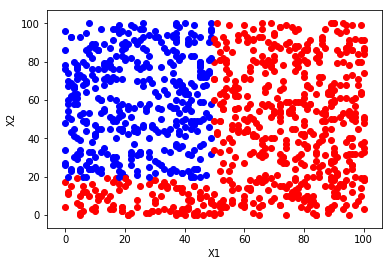
\includegraphics[scale=0.4]{decision_tree_example_data} & \raisebox{.4\height}{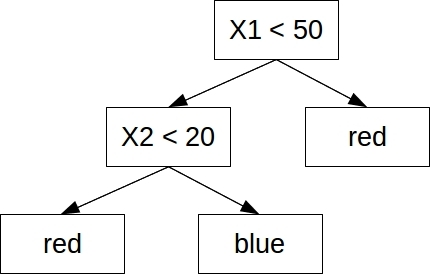
\includegraphics[scale=0.4]{decision_tree_example}}
        \end{tabular}
    \end{center}
    \caption{\label{tab:DecisionTreeExample}Example of Decision Tree}
\end{table}

The algorithms for the construction of decision trees usually work by recursively partitioning the training set $\mathbf{X}$ in such a way that the values of the target vector $\textbf{y}$ are grouped together, until all partitions are composed by a single label. The problem with these building methods is that they produce very complex trees that overfit the training data. Overfitted trees not only lead to poor predictive capabilities on non-training data, but also produce models that can be exceedingly difficult to interpret. A common approach to avoid overfitting in decision trees is to force an early stopping of the algorithm before the tree becomes too complex. Popular stopping criteria include limiting the maximum depth of the tree, requiring a minimum number of sample points at leaf nodes, or computing the accuracy gain yielded by adding new nodes. However, those heuristics demand the optimization of hyperparameters which makes the training process computationally expensive.

    {\color{red} TODO: briefly describe bagging, random forests, and boosting [...] produce multiple trees which are then combined to yield a single consensus prediction [...] combining a large number of trees can often result in dramatic improvement in prediction accuracy, at the expense of some loss of interpretability [...]}

% Subsection: Time Series

\subsection{Time Series Analysis}
\label{sec:intro_time_series}

A time series is a sequence of measurements taken at successively equally spaced points in time, so there exists a natural ordering of the observations. Examples of time series include the daily closing prices of the Standard and Poor's 500 index, the monthly number of passengers of an airline, or the yearly gross domestic product of a particular country. Time series forecasting refers to the process of building a model to predict future values of the series based on the previously observed values. The observed values could be continuous, discrete or even categorical.

{\color{red} Time series are analysed to understand the past and to predict the future [...] A time series analysis quantifies the main features in data and the random variation [...] When a variable is measured sequentially in time over or at a fixed interval, known as the sampling interval, the resulting data form a time series [...] we take a statistical approach in which the historical series are treated as realizations of sequences of random variables [...] referred to as a discrete-time stochastic process [...] The main features of many time series are trends and seasonal variations that can be modelled deterministically with mathematical functions of time. Another important feature of most time series is that observations close toghether in time tend to be correlated (serially dependent) [...] Once a good model is found and fitted to data, the analyst can use the model to forecast future values [...] Fitted models are also used as a basis for statistical tests. [...] Finally, a fitted statistical model provides a concise summary of the main characteristics of a time series. [...] The data may have been aggregated [...] or sampled [...] If data are sampled, the sampling interval must be short enough for the time series to provide a very close approximation to the original continuous signal when it is interpolated [...] a systematic change in a time series that does not appear to be periodic is known as a trend. [...] A repeating pattern [...] within any fixed period [...] is known as seasonal variation [...] cycles [...] do not correspond to some fixed natural period. [...] Forecasting relies on extrapolation, and forecast are generally based on assumption that present trends continue. We cannot check this assumption in any empirical way. [...] ouliers and erroneous vales [...] need to be handled differently in the analysis and must not be included as observation when fitting a model to data. [...] it may be appropiate to consider robust methods of fitting models, which reduce the influence of outliers. [...] it is usually appropiate to remove trends and seasonal effects before comparing multiple series. [...] trend [...] change direction in unpredictable times [...] stochastic trend [...] two unrelated time series will be correlated if they both contain a trend.}

\begin{definition}
    A \emph{time series} of length $n \in \mathbb{N}$, denoted by $\{ x_t : t=1, \ldots, n \}$ or $\{ x_t \}$, is a sequence $\{ x_1, x_2, \ldots, x_n \}$.
\end{definition}

The elements $x_i$ of the series correspond to values sampled at disrete times $1, 2, \ldots, n$, and they can be continuous or categorical. In statistics, a time series is usually modeled as a sequence of $n$ random variables, and a particular time series is a realization of the model. In this sense, $\{ x_t \}$ could represent a collection of random variables or the numerical observations of these random variables.

{\color{red} We represent a time series of length $n$ by $\{ x_t : t=1,\ldots,n \} = \{x_1, x_2, \ldots, x_n \}$. It consists of $n$ values sampled at discrete times $1, 2, \ldots, n$. The notation will be abbreviated to $\{x_t\}$ when the length $n$ of the time series do not need to be specified. The tiem series model is a sequence of random variables, and the observed time series is considered a realizatin of the model.
}

{\color{red} The 'hat' notation will be used to represent a prediction or forecast. For example, with the series $\{ x_t : t=1,\ldots,n \}$, $\hat{x}_{t+k \mid t}$ is a forecast made at time $t$ for a future value at time $t+k$. A forecast is a predicted future value, and the number of time steps into the future is the lead time $k$ [...]
}

\subsubsection{Trends and Seasons}

Many time series ... and a repeating seasonal component.

\begin{definition}
    Let $\{ x_t \}$ be a time series, a \emph{simple additive model} is defined as
    \[
        x_t = m_t + s_t + z_t
    \]
    where $m_t$ is called the \emph{trend component}, $s_t$ is the \emph{seasonal component}, and $z_t$ is the \emph{error term}.
\end{definition}

If the time series presents the property that the seasonal component increases as the trend increases, it might be better to use a multiplicative model.

\begin{definition}
    Let $\{ x_t \}$ be a time series, a \emph{simple multiplicative model} is defined as
    \[
        x_t = m_t \dot s_t + z_t
    \]
    where $m_t$ is called the \emph{trend component}, $s_t$ is the \emph{seasonal component}, and $z_t$ is the \emph{error term}.
\end{definition}

In practice, a simple approach of estimating the trend of a tiem series is to compute a moving average.

\begin{definition}
    Let $\{ x_t \}$ be a time series, a \emph{simple moving average} of lenth $l$ is 
\end{definition}

The best results are achieved when the length $l$ of the moving average is equal to the length of the seasonal component. The seasonal componet can be estimated by

\begin{definition}
    Additive
    \[
        \hat{s}_t = x_t - \hat{m}_t
    \]
    Multiplicative
    \[
        \hat{s}_t = \frac{x_t}{\hat{m}_t}
    \]
\end{definition}


{\color{red} [...] many series are dominated by a trend and/or a seasonal effect [...] A simple additve decomposition model is given by
\[
    x_t = m_t + s_t + z_t
\]
where, a time $t$, $x_t$ is the observed series, $m_t$ is the trend, $_t$ is the seasonal effect, and $z_t$ is an error terms that is, in general, a sequence of correlated random variables with mean zero.

If the seasonal effect tends to increase as the trend increases, a multiplicative model may be more appropriate
\[
    x_t = m_t \dot s_t + z_t
\]

}

\begin{definition}
    
\end{definition}

{\color{red} Once we have identired any trend and seasonal effects, we can deseasonalise the time series and remove the trend. If we use the additive decomposition method, we first calculate the seasonality adjusted time series and then remove the trend by substraction. This leaves the random component, but the random component is not necessarily well modelled by independent random variables. In many cases, consecutive variables will be correlated. If we identify such correlations, we can improve our forecast, quite dramatically if the correlations are high.}

\subsubsection{Second Order Properties}

A possible approach to forecas future values of a time-series based variable is to extrapolate the current trend and to apply some adaptative estimations.


\subsubsection{Exponential Smoothing}

\begin{definition}
Let's $x$ and $y$ two time series. The cross covariance function of $x$ and $y$ as a function of a lag $k$, denoted $\gamma \left( x, y \right)$, is defined as:
\[
    \gamma \left( x, y \right) = E 
\] 

\end{definition}

\begin{definition}

\end{definition}

%
% Autocorrelation, Cross-correlation and Partial Autocorrelation
% 
\subsubsection{Autocorrelation, Cross-correlation and Partial Autocorrelation}

Autocorrelation measures the (Pearson) correlation of a time series with a delayed version of itself, and as a function of that delay. Autocorrelation is intended to estimate the degree of similarity of an observation with respect to previous observations.

\begin{definition}
Let $\{\mathbf{X}_t\}$ be a time series with mean $\mu$ and varianze $\sigma^2$. The lag $k$ \emph{autocorrelation} function, denoted by $\rho$, is defined as:
\[
\rho(k) = \frac{E\left[\left(x_{t}-\mu\right)\left(x_{t+k}-\mu\right)\right]}{\sigma^{2}}
\]
\end{definition}

The autocorrelation function is not defined for all time series, because the mean may not exist (time series with a trend), or the variance may be zero (constant time series). A time series for which the autocorrelation is defined is called \emph{second order stationary}.

The \emph{sample autocorrelation} is computed in practice by:
\[
\hat{\rho}(k) = \frac{ \frac{1}{n}\sum_{t=1}^{n-k}\left(x_{t}-\bar{x}\right)\left(x_{t+k}-\bar{x}\right) }{ \left( \frac{1}{n}\sum_{t=1}^{n}\left(x_{t}-\bar{x}\right) \right)^2 }
\]
On the contrary of what happened with autocorrelation, sample autocorrelation is defined in case of time series with a trend. However, we must be carefull about the interpretation of the results. In general, sample autocorrelation is applied over the residuals of a time series once the trend and the seasonal components have been removed.

A correlogram is a plot of the sample autocorrelations $\hat{\rho}(k)$ versus time lags $k$ (see Figure {\color{red} XXX}). The dotted lines are drawn at $-\frac{1}{n}\pm\frac{2}{\sqrt{n}}$. If $\hat{\rho}(k)$ is outside these lines for a value of $k$ we have evidence against the null hypothesis that $\hat{\rho}(k)=0$ at the $5\%$ level (See Section {\color{red} XXX}). It is expected that $5\%$ of the estimates $\hat{\rho}(k)$ fall outside these lines.

{\color {red} TODO: Insert Figure. If the example is drawn using matplotlib.pyplot.acorr, the above paragraph is not true. Investigate how the shared areas in the correlogram used by matplotlib are computed.}

%
% Minimum Message Length
%
\section{Minimum Message Length}
\label{sec:MML}

The \emph{Minimum Message Length} (MML) is based on the idea that a good theory, or explanation, for a dataset is a small collection of premises under which the data is not surprising. The best theories are those which are short, able to explain most of the data, and with a high accuracy. An \emph{explanation message} is composed by two parts: the fist part comprises all the premises induced from the data, including numerical values; the second part contains all the data that cannot be derived from the premises. The message also assumes the existence of some already known and accepted premises (prior knowledge). Given the prior premises and the message it should be possible to recover the original dataset. According to the MML, theories are not rejected due to contradictory measurements, they only make the second part of the message longer.

In the MML principle, a message is a lossless encoded version of the original data. The first part of the message contains a probabilistic model about the data, and the second part is the data encoded using this model. We are interested in finding the shortest possible explanation message. If the length of the explanation message is longer than the original data, the theory is considered unacceptable.

Bayes' theorem (see Theorem \ref{th:bayes}) states that the probability $P(H \mid E)$ of a hypothesis $H$ given an evidence $E$ is:
\[
    P(H \mid E) = \frac{ P( E \mid H ) P(H) }{ P(E) }
\]
We are interested in finding the hypothesis $H$ with the highest posterior probability $P(H \mid E)$ of being true, assuming a fixed evidence $E$. That is, we are looking for maximize $P( E \mid H ) P(H)$ or, equivalently, maximize $P ( H \wedge E )$.

The \emph{Minimum Message Length} principle (MML for short) is based on the idea that the length of encoding $H \wedge E$ as a binary string using an optimal code is equal to $- \log_2 P ( H \wedge E )$ (see Theorem \ref{th:optimal_codes}). That is:
\[
    l(H \wedge E) = - \log_2 P ( H \wedge E ) = - \log_2 P( E \mid H ) P(H) = - \log_2 P( E \mid H ) - \log_2 P(H)
\]
The most probable model $H$ would be that model that allows us to encode $H \wedge E$ with the shortest possible string. The encoded string would be composed by two parts, a general assertion about the data, and a detailed description of the data assuming that the assertion is true.

Let $\mathbb{X}$ be a discrete set composed by all possible datasets, $\mathcal{X}$ a random variable taking values on $\mathbb{X}$, and $f(X \mid \theta)$ a probability distribution for $\mathcal{X}$ given the parameter $\theta$.

\begin{definition}
    Let $\Theta$ be a discrete set of possibles parameters for $f$ with probability distribution $h(\theta) \, \theta \in \Theta$, and let $\hat\theta \in \Theta$ be an inferred parameter. An \emph{assertion} is the encoded version of $\hat\theta$ using an optimal code given the probability distribution $h$.
\end{definition}

The length of the assertion given an optimal binary code is $- \log_2 h(\hat\theta)$ (see Section {\ref{sec:Optimal-Codes}). Note that $\theta$ could be a single scalar or a vector of values. Moreover, $\theta$ could be related to more than one family of probability distributions $f$.

\begin{definition}
    Let $X \in \mathbb{X}$ be a dataset, and $\hat \theta \in \Theta$ an inferred value for the distribution $f$. A \emph{detail} is the encoded version of $X$ using an optimal code given the probability distribution $f(X \mid \hat\theta)$.
\end{definition}

The length of the detail given an optimal binary code is $- \log_2 f( X \mid \hat\theta )$. That is, the length of the detail is the negative of the log-likelihood of $X$ given $\hat\theta$.

\begin{definition}
    Let $X \in \mathbb{X}$ be a dataset, and $\hat \theta \in \Theta$ an inferred value for the distribution $f$ A \emph{message} for the dataset $X$ given an inference $\hat\theta \in \Theta$ is the concatenation of the assertion for $\hat\theta$ and the corresponding detail for $X$ given $\theta$.
\end{definition}

The length of a message given an optimal binary code is $- \log_2 h \left( \hat\theta \right) - \log_2 f \left( X \mid \hat\theta \right)$. The length of a message allow us, for example, to compare the posterior probabilities of two competing explanations or hypotheses $\hat\theta_1$ and $\hat\theta_2$.

\begin{definition}
    Let $X \in \mathbb{X}$ be a dataset. The \emph{Minimum Message Length} of $X$, denoted by $MML(X)$, is given by:
    \[
        MML(X) = \argmin_{\hat\theta \in \Theta} \left( - \log_2 h \left( \hat\theta \right) - \log_2 f \left( X \mid \hat\theta \right) \right)
    \]

\end{definition}

In practice, the actual messages will not be constructed, since our interest is in the length of the messages, not in their content. It is assumed that the sets $\mathbb{X}$ and $\Theta$ and the functions $f(X \mid \hat\theta)$ and $h(\theta)$ are known a priori, and so, it is not necessary to include them as part of our encoding message.

\begin{example}
    \label{ex:MML}
    Consider an experiment in which we toss a weighted coin $100$ times. Denote by $1$ if we get a face and $0$ a cross, so that each experiment is a binary string of length $100$. Our collection of all possible datasets is $\mathbb{X} = \mathcal{B}^{100}$, $\theta$ is a number in the interval $[0, 1]$, the likelihood $f (X \mid \theta)$ follows a binomial distribution (that is, $f (X \mid \theta) ) = \theta^n (1-\theta)^{100-n}$ where $n$ is the number of faces in $X$), and since we do not know anything about how the coin is weighted, we could assume that $h(\theta)$ is the uniform distribution in the interval $[0, 1]$ (that is, $h(\theta) = 1$ for $\theta \in \Theta$). Under these assumptions, the length of a message for $X$ given an inferred parameter $\hat\theta$ would be:
    \[
        - \log_2 h \left( \hat\theta \right) - \log_2 f \left( X \mid \hat\theta \right) = - n \log_2 \hat\theta - (100-n) \log_2 (1 - \hat\theta)
    \]
    We are interested in finding the value of $\hat\theta$ that minimizes the length of the encoded version of $X$, that is, the minimum message length for $X$.
\end{example}

A Maximum A Posteriori analysis of the experiment in Example \ref{ex:MML} would provide the same inference for $\hat\theta$ than the Minimum Message Length approach. Moreover, given that $h(\theta)$ follows an uniform distribution, a Maximum Likelihood approach would reach exactly the same value for $\hat\theta$.

%
% Minimum Description Length
%
\section{Minimum Description Length}
\label{sec:MDL}

The \emph{Minimum Description Length} (MDL) principle is a reformulation
of the Kolmogorov complexity with the goal to make it applicable to
solve practical problems. MDL explicitly address the two most important
practical limitations of the Kolmogorov complexity: its uncomputability
(in general, the Kolmogorov complexity cannot be computed), and the
large constants involved in the invariance theorem (that makes it
inapplicable to short strings). The approach of MDL to these problems
is to scale down Kolmogorov complexity until it does become applicable:
instead of using general-purpose computer languages, MDL is based
on fixed languages and coding functions.

In contrast to Kolmogorov that states that the complexity of a string
is equal to the length of the shortest program that prints that string,
MDL proposes that our capacity to learn about a string is equivalent
to our ability to compress that string. The idea behind MDL is to
describe a dataset with the help of an hypothesis: the more the hypothesis
fits the data (and here good fit equals learning), the more we can
compress the data given that hypothesis.

In our particular case, we are interested in MDL because it will allow
us to compute the nescience of a topic given a dataset, instead of
requiring a text describing the topic. Thus, given a topic $t$ and
a sample dataset $D=\left\{ x_{1},x_{2},\ldots,x_{n}\right\} $, the
nescience of a particular hypothesis $H$ will be related to the capacity
of that hypothesis to compress the dataset.

MDL comes into two versions, \emph{simplified (two-part code) MDL}
and \emph{refined MDL}. Simplified MDL is easier to understand, and
it will allows us to introduce some important concepts and notation.
The extension of the concept of nescience to datasets will be based
on the refined version of MDL.


    {\color{red} TODO: Explain how this relates to cross entropy}


In this section we are going to introduce the two-part code version
of the minimum description length principle for probabilistic models.

\emph{Given a set of candidate models (a set of probability distributions
    (for example first-order Markov chains) or functions of the same functional
    form (for example the kth degree polynomials)) $\mathcal{H^{\left(\text{1}\right)}},\mathcal{H}^{\left(2\right)},\ldots$
    the simplified,} \emph{two-part version,} \emph{of the} Minimum Description
Length Principle \cite{Gr=0000FC05}\emph{ states that the best point
    hypothesis (a single probability distribution (e.g. a Markov chain
    will all parameters values specified) $H\in\mathcal{H^{\left(\text{1}\right)}}\cup\mathcal{H}^{\left(2\right)}\cup\ldots$
    to explain the data $D=\left(x_{1},\ldots,x_{n}\right)\in\mathcal{X}^{n}$
    is the one that minimizes the sum $L(M)+L(D\mid M)$, where $L(M)$
    is the length (in bits) of the model description, and $L(D\mid M)$
    is the length (in bits) of the data encoded with the help of the hypothesis
    ... there is only one reasonable choice for this code ... the so-called
    Shannon-Fano code ... Each hypothesis $H$ may be viewed as a probability
    distribution over $\mathcal{X}^{n}$. For each such distribution there
    exists a code with length function $L$ such that for all $x^{n}\in\mathcal{X}^{n}$
    we have that $L\left(x^{n}\right)=-\log_{2}P\left(x^{n}\mid H\right)$.
    The quantity $L(M)$ depends on each model.}

\emph{A description of the data ``with the help of'' a hypothesis
    means that the better the hypothesis fits the data, the shorter the
    description will be. A hypothesis that fits the data well gives us
    a lot of information about the data. Such information can always be
    used to compress the data. This is because we only have to code the
    errors the hypothesis makes on the data rather than the full data.}

\emph{The sum of the two description length will be minimized at a
    hypothesis that is quite (but not too) ``simple'', with a good (but
    not perfect) fit.}

The length of the data given the model, that is, \emph{$L(D\mid M)$.}

\[
    -\log P(D)=L_{C}(D)
\]


This choice for C gives a short codelegth to sequences which have
high probability according to (k, ttita) while it gives a high codelength
to sequences with low probability. The codelength thus directly reflects
the goodness-of-fit of the data with respect to (k,tita) measured
in terms of the probability fo D according to (k,tita).

When we say we ``code the data D with the help of probabilistic hypothesis
P'' we mean that we code D using the Shannon-Fano code corresponding
to P.

\[
    L(D\mid P):=-\log P(D)
\]


the code with these lengths is the only one that would be optimal
if P where true. (mention we are only interested in code lengths,
we are not interested in to find the code itself).

For \emph{$L(M)$ we use the standard code for integers.}

\begin{example}
    Markov Chain Hypothesis Selection: Suppose we are given data $D X\textasciicircum{}n$
    where $X=\{0,1\}$. We seek a reasonable model for D that allows us to
    make good predictions of future data coming from the same source.
    We decide to model our data using the cass B o all Markov chains ${[}...{]}$
    we face the problem of overfitting: for a given sequence $D=(x1,...,xn)$,
    there may be a Markov chain P of very high order that fits data D
    quite well but that will behave very badly when predicting future
    data from the same source.
\end{example}

\subsection{Refined MDL}

\emph{In refined MDL, we associate a code for encoding $D$ not with
    a single $H\in\mathcal{H}$ but with the full model $\mathcal{H}$
    ... we design a single one-part code with lengths $\bar{L}\left(D\mid H\right)$
    (called the stochastic complexity of the data given the model). This
    code is designed such that whenever there is a member of (parameter
    in) $\mathcal{H}$ that fits the data well, in the sense the $L\left(D\mid H\right)$
    is small, then the codelenth $\bar{L}\left(D\mid H\right)$ will also
    be small. Codes with this property are called universal codes.}

\emph{There are at least four types of universal codes:}
\begin{enumerate}
    \item \emph{The normalized maximum likelihood (NML) code and its variations.}
    \item \emph{The Bayesian mixture code and its variations.}
    \item \emph{The prequential plug-in code.}
    \item \emph{The two-part code.}
\end{enumerate}
\emph{Refined MDL is a general theory of inductive inference based
    on universal codes that are designed to be minimax, or close to minimax
    optimal. It has mostly been developed for model selection, estimation
    and prediction.}

\section{Multiobjective Optimization}

In the area of \emph{multiobjective optimization} we are interested in solving the following problem:
\begin{align*}
     & \text{minimize}	   \quad \left\{f_1(x), f_2(x), \ldots, f_k(x) \right\} \\
     & \text{subject\;to} \quad x \in S
\end{align*}
where $f_i:\mathbb{R}^n \rightarrow \mathbb{R}$ are two or more objective \emph{objective functions}, and the nonempty set $S \subset \mathbb{R}^n$ is the \emph{feasible region}, whose elements $x=\left( x_1, x_2, \ldots, x_n \right)$ are \emph{decision vectors}. The image of the feasible region $f(S) \subset \mathbb{R}^k$ is called \emph{objective region}, and its elements $z = \left(f_1(x), f_2(x), \ldots, f_k(x) \right)$ \emph{objective vectors}.

In this book we will be dealing with nonlinear multiobjective optimization problems, where at at least one of the objective functions is not linear. Objective functions can be also incommensurable, that is, measured in different units.

An objective vector is optimal if none of its components can be improved without deteriorating at least one of the others. In multiobjective optimization the objective functions are usually conflicting, and so, it does not exist a single solution that is optimal with respect to every objective function.

\begin{definition}
    A decision vector $x \in S$ is Pareto optimal if there does not exists another decision vector $y \in S$ such that $f_i(y) \leq f_i(x)$ for all $i = 1, \ldots, k$ and $f_j(y) < f_j(x)$ for at least one $j$. An objective vector $z \in f(S)$ is Pareto optimal if there does not exits another objective vector $w \in f(S)$ such that $w_i \leq z_i$ for all $i = 1, \ldots, k$ and $w_j < z_j$ for at least one $j$.
\end{definition}

An objective vector is Pareto optimal if its corresponding decision vector is Pareto optimal.

    {\color{red} [...] the Pareto optimal set (consisting of the Pareto optimal solutions) can be nonconvex and disconnected [...]}

    {\color{red} TODO: Add an example}

    {\color{red} [...] in practice, usually only one of these solutions is to be chosen [...] In multiobjective optimization, there are at least two equally important tasks: an optimization task for finding Pareto optimal solutions [...] and a decision-making task for choosing a single most preferred solution}

    {\color{red} [...] putting the preference articulation stage after optimization [...]}

    {\color{red} TODO: Introduce the following concepts: locally Pareto optimal, weak Pareto optimality}

    {\color{red} TODO: Introduce the following concepts: ideal vector (lower bound), nadir (upper bound), utopian}

    {\color{red} TODO: Indroduce the following concept: Decision Maker [...] because Pareto optimal solutions cannot be ordered completely, we need extra preference information coming from a decision maker [...] explicit preference model [...]}

    {\color{red} [...]there is no DN and his preference information available and in those cases we must use so-called no-preference methods. Then, the task is to find some neutral compromise solution without any additional preference information. This means that instead of asking the DM for preference information, some assumptions are made about what a "reasonable" compromise could be}

\subsection{Trade-offs}

{\color{red} [...] a trade-off is an exchange, that is, a loss in one aspect of the problem, in order to gain additional benefit in another aspect [...] a trade-off represents giving up in one of the objectives, which allows the improvement of another objective [...] how much must we give up of a certain objective in order to improve another one to a certain quantity}

{\color{red} objective trade-off vs. subjective trade-off}

{\color{red}

    \begin{definition}
        Let us consider two feasible solutions $x^1$ and $x^2$, and the corresponding objective vectors $f(x^1)$ and $f(x^2)$. Then, the ratio of change between $f_i$ and $f_j$ is denoted by $T_{ij}$
    \end{definition}

}

\subsection{Optimization Methods}

{\color{red} Sometimes, there is no DM and his preference information available and in those cases we must use so-called no-preference methods. Then, the task is to find some neutral compromise solution without any additional preference information. This means that instead of asking the DM for preference information, some assumptions are maked about what a "reasonable" compromise could be like.}

{\color{red} it is important that the multiobjective optimization method used can meet the following two needs: firstly, it must be able to cover, that is, find any Pareto optimal solution, and, secondly, generate only Pareto optimal solutions.}

%
% Section: References
%

\section*{References}

 {\color{red} TODO: Add paper of Turing about AI.}

The minimum message length principle was developed by Chris Wallace, published for first time in 1968 in \cite{wallace1968information}. The book \cite{wallace2005statistical}, written by the same author, contains a detailed description of the principle.

